
%
% derived from the DAFx-06 templates
% derived from the ICMC 2009 templates by Steve Beck
% and then derived from the ICMC 2010 template
% 1) Please compile using latex or pdflatex.
% 2) Please use figures in vectorial format (.pdf); .png or .jpg are working otherwise 
% 3) Please use the "papertitle" and "pdfauthor" commands defined below

%------------------------------------------------------------------------------------------
\documentclass[twoside,10pt,a4paper]{article}
\usepackage{icmc2011,amssymb,amsmath} 
%\setcounter{page}{1}

\usepackage{mathptmx} 

%____________________________________________________________
%  !  !  !  !  !  !  !  !  !  !  !  ! user defined variables  !  !  !  !  !  !  !  !  !  !  !  !  !  !
%==== set the title ====
\def\papertitle{Gesture Analysis of radiodrum data}
%\def\papertitle{}	%-- should be empty for the submission anyway!

%==== 1st submission: author name and affiliation are empty for anonymous submission ====
\def\paperauthorA{tet} 
\affiliation{}{}


%==== final submission: author name and affiliation ====
%---- uncomment 1 to 4 lines, for 1 to 4 authors
\def\paperauthorA{Steven R. Ness}
\def\paperauthorB{Sonmaz Zehtabi}
\def\paperauthorC{Andrew W. Schloss}
\def\paperauthorD{George Tzanetakis}

%%---- set correspnding affiliation data for...
%%-- 1 author
%\affiliation{\paperauthorA}
%  {School\\ Department, City, Country \\ {\tt \href{mailto:email@domain.icmc}{email@domain.icmc}}}

%%-- 2 authors with same affiliation
%\affiliation{\paperauthorA, \paperauthorB}
%  {School\\ Department, City, Country \\ {\tt \href{mailto:email@domain.icmc}{email@domain.icmc}}}

%-- 2 authors with different affiliations
\twoaffiliations{\paperauthorA, \paperauthorB, \paperauthorD}{University of Victoria\\ Department of Computer Science}
  {\paperauthorC}{University of Victoria\\ School of Music}

%%-- 3 authors with different affiliations
%\threeaffiliations{\paperauthorA}{School A\\ Department X}
%  {\paperauthorB}{Company\\ Address}
%  {\paperauthorC}{School B\\ Department Y}

%-- 4 authors with different affiliations
% sness - Had to hack this to get the spacing to work out right
%% \fouraffiliations
%%  	{\paperauthorA \ \ \ }{University of Victoria\\ Department of Computer Science}
%%  	{\paperauthorB}{University of Victoria\\ Department of Computer Science}
%%  	{ \ \ \ \paperauthorC\ \ \ \ \ \ \ }{\ \ \ \ \ \ University of Victoria \ \ \ \ \ \ \ \ \ \ \\ \ \ \ \ \ \  \ \ \ \ \ \ \ School of Music\ \ \ \ \ \ \ \ \ \ \ \ \ \ \ \ \ \  }
%%  	{\paperauthorD}{University of Victoria\\ Department of Computer Science}

%% \threeaffiliations
%%  	{\paperauthorA, \paperauthorB}{University of Victoria\\ Department of Computer Science}
%%  	{\paperauthorC}{University of Victoria\\ School of Music}
%%  	{\paperauthorD}{University of Victoria\\ Department of Computer Science}

%  ^  ^  ^  ^  ^  ^  ^  ^  ^  ^ user defined variables  ^  ^  ^  ^  ^  ^  ^  ^  ^  ^  ^  ^ 
%------------------------------------------------------------------------------------------

%%-- if using .ps or .eps figure files, they will be converted on the fly
%%-- RMK: for faster LaTeX runs, use it only once after adding new \includegraphics[]{} cmds
%\usepackage{epstopdf}	 

%---- the hyperref package must be last to properly work
%% \usepackage[pdftex,
%%        pdftitle={\papertitle},
%% 	pdfauthor={\paperauthorA},
%% 	colorlinks=false,bookmarksnumbered,pdfstartview=XYZ]{hyperref}
%% \usepackage[pdftex,
%%        pdftitle={\papertitle},
%% 	pdfauthor={\paperauthorA},
%% 	colorlinks=false,bookmarksnumbered,pdfstartview=XYZ]
%\pdfcompresslevel=9
\usepackage[pdftex]{graphicx}	% for compatible graphics with hyperref
%% \usepackage[figure,table]{hypcap}	% corrects the hyper-anchor of figures/tables

\title{\papertitle}

%------------------------------------------------------------------------------------------

\renewcommand\floatpagefraction{.9}
\renewcommand\topfraction{.9}
\renewcommand\bottomfraction{.9}
\renewcommand\textfraction{.1}   
\setcounter{totalnumber}{50}
\setcounter{topnumber}{50}
\setcounter{bottomnumber}{50}

\begin{document}

\DeclareGraphicsExtensions{.png,.jpg,.pdf} % used graphic file format for pdflatex
    
\maketitle

\begin{abstract}
The radiodrum is a virtual controller/interface that has existed in
various forms since its initial design at Bell Laboratories in the
1980's, and it is still being developed.  It is a percussion
instrument, while at the same time an abstract 3D gesture/position
sensor.  There are two main modalities of the instrument that are used
by composers and performers: the first is similar to a percussive
interface, where the performer hits the surface, and the instrument
reports position (x,y,z) and velocity (u) of the hit; thereby it has 6
degrees of freedom.  The other mode, which is unique to this
instrument (at least in the domain of percussive interfaces), is
moving the sticks in the space above the pad, whereby the instrument
also reports (x,y,z) position in space above the surface.

In this paper we describe techniques for identifying different
gestures using the Radio Drum, which could include signals like a
circle or square, or other physically intuitive gestures, like the
pinch-to-zoom metaphor used on mobile devices such as the iPhone. Two
approaches to gesture analysis are explored. The first one is based on
feature classification using support vector machines and the second is
using Dynamic Time Warping. By allowing users to interact with the
system using a complex set of gestures, we have produced a system that
will allow for a richer vocabulary for composers and performers of
electro-acoustic music.  These techniques and vocabulary are useful
not only for this particular instrument, but can be modified for other
3D sensors.

\end{abstract}

\section{Introduction}\label{sec:introduction}

The radiodrum \cite{schloss89} \cite{tindale05} is a virtual
controller/interface that has existed in various forms since its
initial design at Bell Laboratories in the 1980's, and it is still
being developed.  Using capacitive sensing, it can detect the position
of two augmented drum sticks in a space above a receiver antenna.  It
is a percussion instrument, while at the same time an abstract 3D
gesture/position sensor.  Currently, there are two modes of
interaction: the first is similar to a percussive interface, where the
performer hits the surface, and the instrument reports position (x,y,z)
and velocity (u) of the hit; thereby it has 6 degrees of freedom.  We
call this ``whack'' mode.  Note that this mode does not depend on
hitting the surface; it is detected by the change of direction of the
stick and not by any impact as in conventional drum pads.  The other
mode, which we call ``continuous'' mode, is unique to this instrument
(at least in the domain of percussive interfaces).  This mode involves
moving the sticks through space above the pad, whereby the instrument
also reports (x,y,z) position in space above the surface at any
desired sampling rate.

In the current work we propose to extend the radiodrum with a new
modality of interaction with a system that recognizes gestures made by
the performer.  These gestures can be as simple as a sweep across the
surface of the radiodrum, or can be as complex as the composer or
performer desires.  These gestures are then sent to a system the
produces sound or image, for example, a Max/MSP \cite{puckette02}
patch.  These gestures can either be mapped to actions that send
metadata to the patch, for example, a different section of a musical
piece could be triggered, or can be mapped directly to sound producing
modules.  In the case of a direct mapping to sound, the speed of the
gesture itself could be mapped to musical properties of the sound.

\section{Background}

The word gesture is a highly overloaded term, and has a variety of
meanings in a number of different fields.  Because of this, the
concept of gesture can be viewed as a boundary object \cite{star89},
that is, a concept that is at once adaptable to different viewpoints,
but also robust enough to maintain its identity across different
fields.  A detailed examination of gestures can be found in Cadoz and
Wanderley \cite{cadoz00}, where they categorize gestures in music as
effective gestures, accompanist gesture and figurative gestures.  The
gestures detected by our system fall into all three of these
categories.  In a review by Overholt \cite{overholt07}, three basic
groups of gestural controllers for music are summarized, which include
those inspired by instruments, augmented instruments and alternative
instruments.  Our system is inspired by drums, but can also be viewed
as an augmented drum.

\section{Related Work}

There have been many approaches to detecting gestures in the current
literature.  These include computer vision based methods, and
approaches using accelerometer data. Early work in the field of
gesture recognition employed the concept of Space-time gestures
\cite{darrell93} in which sets of view models are captured by a
Computer Vision system and are matched to stored gesture patterns
using Dynamic Time Warping (DTW). Although this system was not used to
produce music, it is relevant to the current work because it uses the
same technique of Dynamic Time Warping to recognize patterns in a
multi-dimensional space.

Another more recent paper \cite{corradini01} also uses DTW for the
recognition of a small gesture library, in a non-realtime setting.  It
takes hand-arm gestures from a small, predefined vocabulary and uses a
DTW engine to align these gestures in time and also to perform
normalization on them. 

More relevant to the current work are papers that perform gesture
recognition on the data from accelerometers, such as those now
commonly found on devices such as the iPhone and Wii-mote.  An early
work in this field was described in ``SICIB: An Interactive Music
Composition System Using Body Movements'' \cite{moralesmanzanares01}
where a rule based coupling mechanism linking the position, velocity,
acceleration, curvature, torsion of movements and jumps of dancers is
mapped to intensity and tone in music sequences.

Another recent paper relevant to current work describes
uWave\cite{liu09}, an accelerometer-based personalized gesture based
system.  This system is unusual in that the system uses a single
prototypical example of each gesture, and uses DTW to recognize a
simple gesture vocabulary containing eight signs, derived from the
Nokia gesture alphabet. Akl et al. \cite{akl10} describe an approach
that extends this work using DTW, affinity propagation and compressive
sensing.  In this paper, 18 gestures are recognized, as opposed to 8
for the uWave\cite{liu09} paper.  The addition of compressive sensing
allows gestures to be reduced to a more sparse representation that is
then matched using DTW.

Another interesting new approach \cite{wu09} does not use either DTW
or heuristics, but instead uses the machine learning technique of
Support Vector Machines (SVM) and does gesture recognition with 3D
accelerometer data.  In this paper, a system that uses a frame-based
descriptor and a multi-class SVM is described.  With frame-based
descriptors, instead of using the entire time series, a reduced
representation is used, and in this paper, spectral descriptors
calculated by a Fast Fourier Transform are used.  This paper describes
how this approach outperforms DTW, Naive Bayes, C4.5 and Hidden Markov
Model (HMM) machine learning systems.

The approaches described in the previous paragraphs have positive
attributes as well as challenges.  Computer vision based approaches
have the advantage that electronic cameras are now cheap commodity
hardware and are easily available.  However, computer vision based
approaches are fundamentally limited by their hardware requirements of
cameras and transmitters and high computational load \cite{liu09}.
They also have a low acquisition framerate as compared to other
approaches.

%% Smart glove based solutions can recognize very fine gestures but
%% require the user to wear a glove tagged with multiple sensors to
%% capture finger and hand motions in fine granularity \cite{liu09}.
%% They also require a high overhead of engagement with the user.

Accelerometer based approaches have the advantage that with MEMS
technology small cheap solutions are becoming common \cite{wu09} and
they provide a high speed and continuous source of data, ideal for
machine learning approaches.  However, accelerometers suffers from
abrupt changes due to hand shaking\cite{akl10}.

In the past three years, we collaborated with Bob Boie, the original
designer of the radiodrum at Bell Labs in the 1980's, in the design of
a new instrument that does not use MIDI at all.  Boie worked with Max
Mathews in the 1980's, and is known for being one of the original
designers of capacitive sensing tablets, including very early versions
of trackpads and similar devices.  There is considerable confusion in
the computer music community about the radiodrum vs. Radio Drum
vs. Radio Baton and the history thereof.  We will not go into detail
here, but suffice it to say that this new instrument is more accurate
and satisfying to use in performance that the older versions.  At the
moment, we only have one prototype, but we are in the process of
building more instruments.

MIDI works reasonably well for asynchronous data like drum-hits, but
it is badly suited for continuous position data.  The new instrument
that Boie designed is entirely analog, and we collect data from it by
amplitude-modulating the analog sensor data in order to take it out of
the DC frequency range.  Then we digitize it using an ordinary audio
interface, and this allows us to use almost any sampling rate so we
get very precise temporal data with no jitter or throughput issues,
orders of magnitude faster than data obtained by computer vision
techniques.

Our radiodrum-based approach has the advantage that absolute position
data is transmitted, and these data are in the form of (x,y,z)
three-tuples that have a direct relation to the position of the sticks
in the real world. They also have the advantage that extremely high
rates of data with excellent time resolution can be obtained.  Since
the radiodrum is a 3D sensor, we know exactly where the sticks are at
all times, not just when they strike the surface.


\section{System Description}

Our system works by matching gestures to a library of template
gestures, usually provided by the performer or composer.  It then
performs real-time matching of gesture data from the radiodrum in the
form of a list of tuples of x,y,z values and matches this stream of
data to the template library, returning the matching template gesture.

The mapping of gestures to sounds is in the domain of the composer,
who in our system would be responsible for creating this mapping of
gestures to sounds. To use our system, the composer and performer
would define an alphabet of gestures that will be used.

During the performance of the piece of music, when the musician wants
a gesture to be recognized, they then push a foot switch which
activates the gesture recognition system, and then execute a gesture.
A similarity matrix between this gesture and all examples of all
gestures in the system is then calculated.  A similarity matrix of two
examples of the gesture for ``A'' is shown in Figure \ref{fig:a0-a1}.

\begin{figure}[htb]
\begin{center}
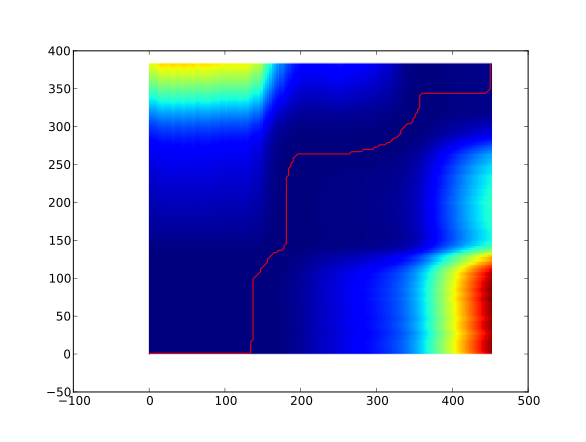
\includegraphics[width=80mm]{a0-a1}
\end{center}
\caption{
Similarity matrix for two examples of the sign ``A'' along with the
best path as determined by Dynamic Time Warping shown in red.}
\label{fig:a0-a1} 
\end{figure} 

\section{Results}

We have implemented two independent systems for doing gesture
recognition of radiodrum data.  The first of these is a system based
on Dynamic Time Warping (DTW) \cite{darrell93} and the second is a
system based on a frame based implementation using a Support Vector
Machine (SVM) machine learning classifier.

\subsection{Dynamic Time Warping}

In our DTW implementation, we take the X and Y pairs of a performed
gesture and compare each of the X and Y time series to all the
examples of the gesture in our gesture alphabet.  Specifically, we
first take the X time series of the performed gesture and calculate a
similarity matrix between all points of this gesture and each gesture
in our database.  We then run the DTW algorithm on this
similarity matrix and find the cost of the path as determined by the
DTW algorithm, where a lower cost path indicates a more likely gesture
match.  We then repeat this for the Y time series and sum the scores
for the X and Y values.  The lowest cost path over all the gestures in
our alphabet is then returned as the most likely match.

We performed a series of experiments to evaluate the performance of
the DTW algorithm.  For the first of these, we compared three very
distinct signs, those of ``A'', ``K'' and ``C'' as used in the Palm
Pilot graffiti alphabet.  Exemplars of these three letters are shown
in Figure \ref{fig:ack}.  We took 8 to 10 examples of each of these
letters and performed DTW against all 30 examples in the gesture
database.  We then calculated the precision and recall of the top 8
returned gestures.  The results of this experiment are shown in Table
\ref{table:precisionrecall}.  As one can see, the precision for each
of these is high, for A and K the precision is 1, which means all of
the 8 returned gestures matched the query gesture correctly.  For all
three examples, the recall was also high, and varied between 0.727 and
0.888.  In addition, for all three gestures the top result (Top-1) was
correct in all cases, this is the most important measure because it
matches more closely the behaviour of the system in a performance
implementation.

In doing these experiments we noticed that we can get a higher recall
and consequently a higher F-Measure if we specify a cut-off threshold
for DTW score, since this way we eliminate more irrelevant gestures in
the retrieved gestures set. In order to investigate this further,
first we found the optimum threshold for a training set and then to
evaluate the system with obtained thresholds, we tested the system on
the testing set and the result is shown in Table 2
\ref{table:fmeasuretraining}.


\subsection{Support Vector Machine}

In order to extract features for each gesture, first, we divided each
gesture into N equal sized segments.  Then frames are formed by
putting two adjacent segments (each with the length $Ls = L/(N)$)
together and in a way that every two adjacent frame have a segment in
common. In other words, the frame $i$ consists of the segments i and
segment $i + 1$. So, we have $N -1$ frames each with the length $2*Ls$
and each frame consists of two time series axis $x_t$ and $y_t$. The
feature vector of each gesture consists of the feature vectors of all of
its frames. So if the feature vector of the frame i is called $f_i$ then
the feature vector of each gesture is: $F=f_0+ ...+ f_{N-1}$.  So we need
to calculate the feature vector of each frame. In order to do that we
input the x and y axis into FFT function separately, and in the
frequency domain, we calculated the mean and the energy feature:

\[ Mean =\mu_{T,K} = t_{T,K0}^0 \]

\[ Energy = \epsilon_{T,k} = \frac{\sum_{n=1}^{Ls,2-1}|t_{T,k}^n|^2}{|Ls,2-1|} \]

Where the vector t is the output of the FFT function, $T\ =\ x,\ y\ and\ k
=0,...,N-1$.  After calculating the features for all the frames, we
end up with the feature vector of the gesture:

\[ \tau = ( \mu_{T,K},\epsilon{T,k}) \]

Now the gesture i can be represented by $(g_i , \tau_i)$ and fed to the
binary SVM to train the classifier to recognize the new features.

In this experiment, we first trained the classifier with the training
set that includes 7 samples of the gesture ``A'' and 7 samples of the
gesture ``B''. Then in order to evaluate the model, we used a test set
including 3 samples of the gesture ``A'' and 3 samples of the gesture
``B''.

We repeated this operation for 10 different number of Ns, and three
pairs of gestures (a,b), (c,o) and (k,x).  The results are shown in
Table \ref{table:svm}.  From this table it can be seen that by
choosing the right frame size of the SVM classifier it is possible for
this SVM method to outperform the DTW method.

\begin{table} 
\begin{tabular}{|l|l|l|l|}
\hline
 Gesture   &  Precision  &  Recall & Top-1  \\
\hline
A & 1.0 & 0.888 & 9/9 \\
B & 1.0 & 1.0 & 10/10 \\
K & 1.0 & 0.727 & 10/10 \\
C & 0.792 & 0.704 & 8/8 \\ 
E & 0.818 & 0.595 & 10/10 \\
O & 1.0   & 0.889 & 10/10 \\
\hline
\end{tabular}
\caption{Precision and Recall for three different gestures}
\label{table:precisionrecall}
\end{table}

\begin{table} 
\begin{tabular}{|l|c|c|c|}
\hline
Threshold & F-measure & F-measure & F-measure \\
          &   ``A'' &  ``K'' &  ``O '' \\
\hline
0.020 & 0.966 & 0.927 & 0.982 \\
0.030 & 0.974 & 0.949 & 0.988 \\
0.031 & 0.974 & 0.951 & 0.989 \\
0.036 & 0.967 & 0.952 & 0.990 \\
0.042 & 0.952 & 0.947 & 0.992 \\
0.050 & 0.921 & 0.929 & 0.986 \\
\hline
\end{tabular}
\caption{F-measure for 3 different signs at a variety of training cutoff levels}
\label{table:fmeasuretraining}
\end{table}

\begin{table} 
\begin{tabular}{|l|l|l|l|}
\hline
Frames & Precision & Precision & Precision \\
       & A,B & C,O & K,E \\
\hline
2    & 1.0    & 0.75    & 1.0     \\
4    & 1.0    & 0.66    & 1.0     \\
6    & 0.75   & 1.0     & 1.0     \\
8    & 1.0    & 1.0     & 1.0     \\
10   & 1.0    & 1.0     & 1.0     \\
DTW  & 1.0    & 0.972   & 0.983   \\
\hline
\end{tabular}
\caption{Average Precision and Recall when using the Support Vector
  Machine testing/training approach to gesture recognition.  Shown in
  the last line of the table are the average results for the DTW
  algorithm.}
\label{table:svm}
\end{table}

\begin{figure}[htb]
\begin{center}
\includegraphics[width=80mm]{ack}
\end{center}
\caption{
Exemplars of the gestures ``A'', ``C'' and ``K'' as X,Y pairs of data,
with the Z axis flattened to the plane of the page.}
\label{fig:ack} 
\end{figure} 

\section{Discussion}

Our system is designed for a professional percussionist for live
performances, and thus time and care can be spent in optimizing the
dictionary of signs.  This would also be dependent on the piece of
music and the importance of distinguishing similar signs.  

Data from an accelerometer suffers from abrupt changes due to hand
shaking \cite{akl10}.  In our case, the user moves a stick through
space, and the added mass of the stick helps to mitigate this.  In
addition, this system is intended to be used by experienced
percussionists, who are trained to have good hand coordination when
using percussion mallets or sticks, this fact is indirectly utilized
by our system because we use actual drum sticks that are augmented by
the addition of a small antenna.

Musicians are specifically trained to produce repeatable actions in
order to create sounds.  By using a natural interface for
percussionists, that of a drum stick, we leverage the large amounts of
training that these musicians undergo.

\bibliographystyle{IEEEtranS}
\bibliography{icmc2011gesturesgtzan} 

\end{document}
